
%(BEGIN_QUESTION)
% Copyright 2007, Tony R. Kuphaldt, released under the Creative Commons Attribution License (v 1.0)
% This means you may do almost anything with this work of mine, so long as you give me proper credit

``Smart'' control valve positioners are devices that take a 4-20 mA DC analog current signal and very precisely position the valve stem according to that signal.  Since smart positioners contain microprocessors, they are more than capable of communicating via a digital network standard such as HART.  

A problem may arise, though, if we try to connect more than one HART-capable valve positioner in the same 4-20 mA current loop, such as when we wish to {\it split-range} two or more control valves.  This is where multiple control valves actuate over different portions of the 4-20 mA range, for example a heating valve that operates from 4 to 12 mA and a cooling valve that operates from 12 to 20 mA.  In a traditional (analog) split-range control valve system, the I/P transducers would simply be connected in series so that the same current flowed through both I/P coils, driving both control valves.  With HART-capable positioners, though, we might not want the devices to be connected directly in series, because then there may be a conflict of HART signals when we just wish to ``talk'' with one of the devices.

Explain how this problem is overcome in the following split-range control valve system:

$$\includegraphics[width=15.5cm]{i02230x01.eps}$$

\vskip 20pt \vbox{\hrule \hbox{\strut \vrule{} {\bf Suggestions for Socratic discussion} \vrule} \hrule}

\begin{itemize}
\item{} If we were to connect a HART communicator device to terminals 3 and 4 of TB-1, which control valve would we be communicating with?
\item{} Which valve carries the cooling fluid and which valve carries the heating fluid in this temperature control system?
\end{itemize}

\underbar{file i02230}
%(END_QUESTION)





%(BEGIN_ANSWER)

The HART isolator filters out HART signals to or from one positioner from getting to the other positioner.

\vskip 10pt

We {\it might} communicate with control valve TV-1b, depending on the high-frequency AC characteristics of the controller output.  Certainly, the isolator prevents us from communicating with TV-1a, so we know we can't talk to it.  However, the only way we can talk to the other valve from these connection points is if the HART signals are able to ``pass through'' the controller output.  If the controller output acts as an ideal current source, it should block the HART signals completely, and our communicator will talk to no valve at all.

\vskip 10pt

Control valve TV-1a carries the cooling fluid while control valve TV-1b carries the heating fluid.  As process temperature rises, the reverse-acting controller decreases its output signal.  This will drive TV-1a further open and TV-1b further shut.

%(END_ANSWER)





%(BEGIN_NOTES)


%INDEX% Fieldbus, HART: split-ranging HART valve positioners

%(END_NOTES)


